\documentclass[border=10pt]{standalone}
\usepackage[svgnames]{xcolor}
\usepackage{amsmath}
\usepackage{pgfplots}
\pgfplotsset{compat=newest}
\usepackage[sfdefault]{FiraSans}
\usepackage{FiraMono}
\renewcommand*\familydefault{\sfdefault}
\begin{document}
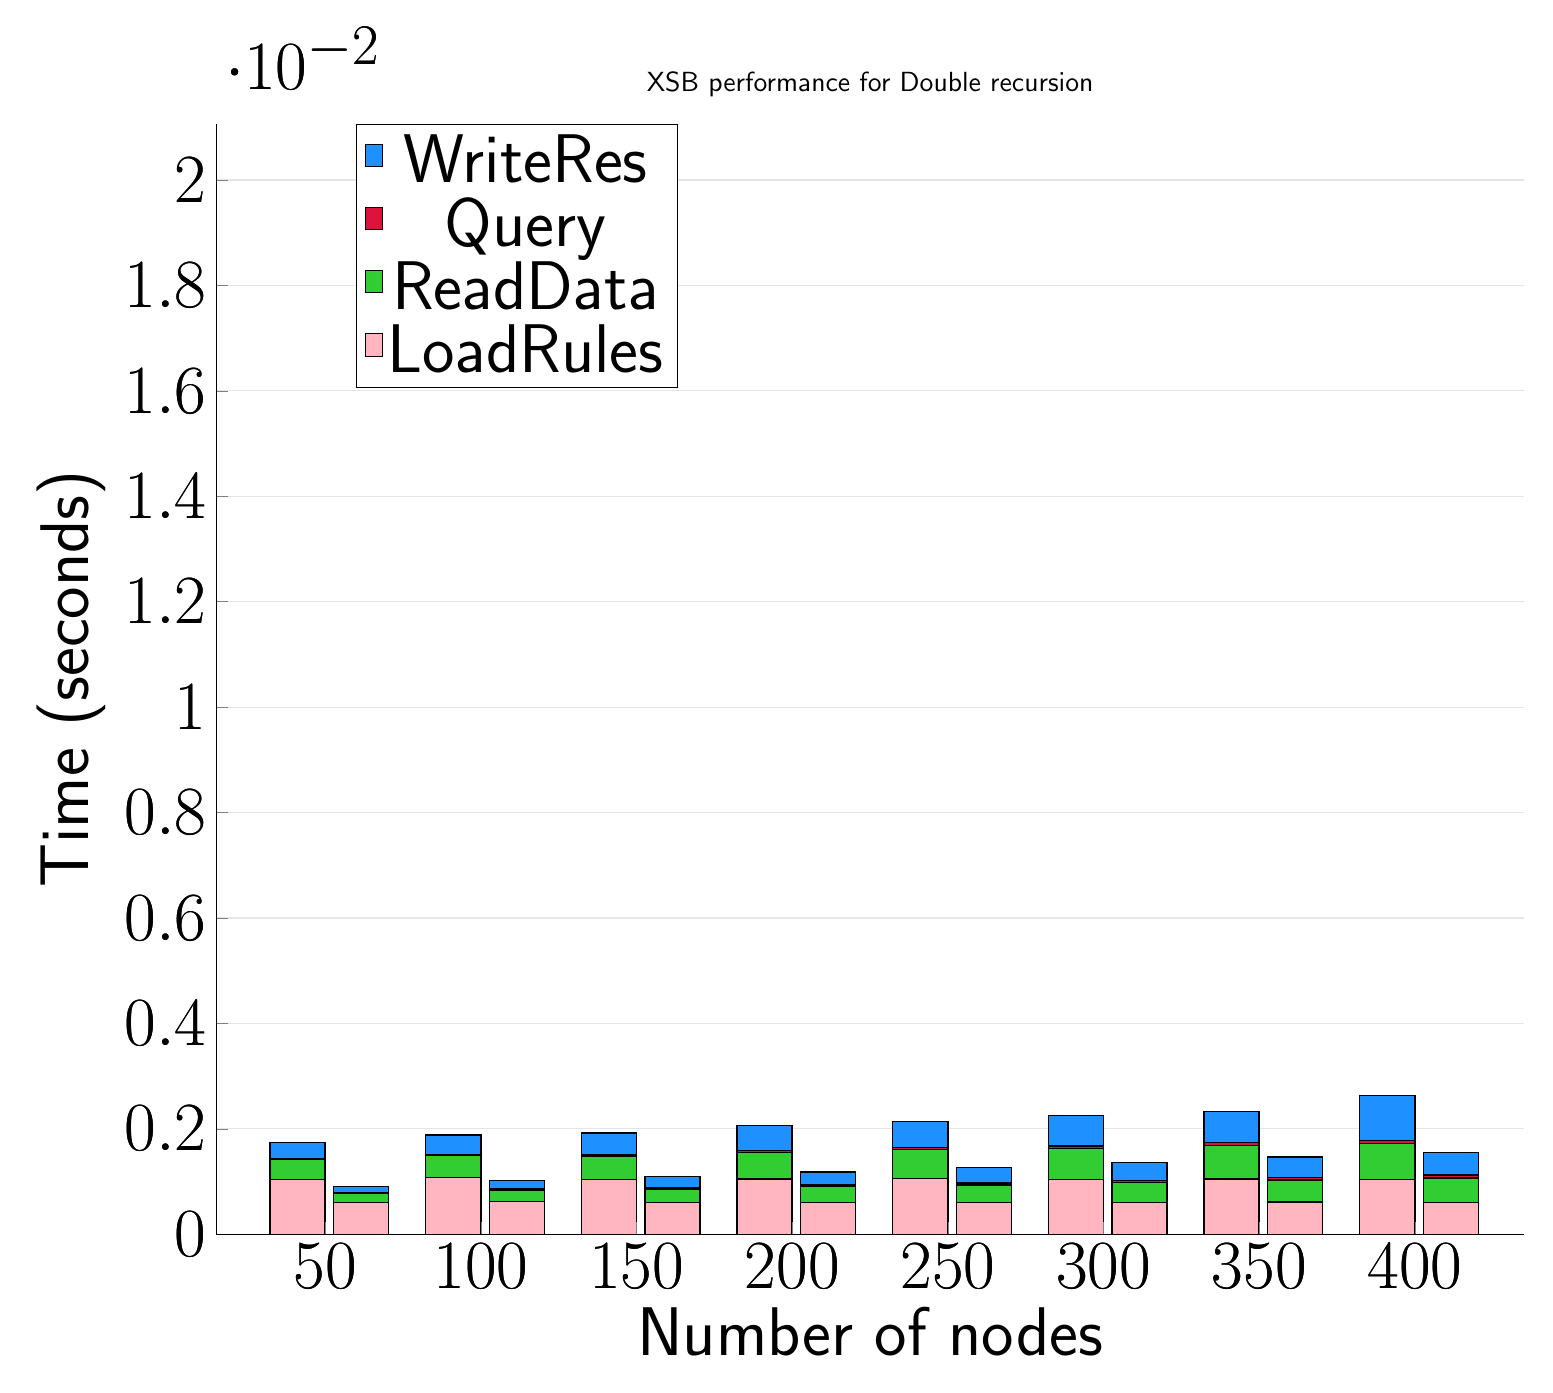
\begin{tikzpicture}
	\begin{axis}[
			ybar stacked,
			title={XSB performance for Double recursion},
			bar shift=-10pt,
			width=1.5\textwidth,
			bar width=0.7cm,
			ymajorgrids, tick align=inside,
			major grid style={draw=gray!20},
			xtick=data,
			ymin=0, ymax=0.021072192192077635,
			axis x line*=bottom,
			axis y line*=left,
			enlarge x limits=0.1,
			legend style={
					at={(0.23, 1)},
					anchor=north,
					legend columns=1,
					font=\Huge,
				},
			ylabel={Time (seconds)},
			xlabel={Number of nodes},
			label style={font=\Huge},
			tick label style={font=\Huge},
		]
		\addlegendimage{fill=DodgerBlue, draw=black, line width=0.2pt}
		\addlegendentry{WriteRes}
		\addlegendimage{fill=Crimson, draw=black, line width=0.2pt}
		\addlegendentry{Query}
		\addlegendimage{fill=LimeGreen, draw=black, line width=0.2pt}
		\addlegendentry{ReadData}
		\addlegendimage{fill=LightPink, draw=black, line width=0.2pt}
		\addlegendentry{LoadRules}
		\addplot +[fill=LightPink, draw=black, line width=0.5pt] coordinates {
				(50, 0.001042795181274414)
				(100, 0.001072192192077636)
				(150, 0.00104360580444336)
				(200, 0.001045227050781251)
				(250, 0.001057004928588867)
				(300, 0.0010404348373413079)
				(350, 0.0010476589202880861)
				(400, 0.001035785675048827)
			};
		\addplot +[fill=LimeGreen, draw=black, line width=0.5pt] coordinates {
				(50, 0.00036962032318115217)
				(100, 0.0004176616668701172)
				(150, 0.00043890476226806643)
				(200, 0.0005068778991699218)
				(250, 0.0005513191223144531)
				(300, 0.0005861282348632813)
				(350, 0.0006398200988769531)
				(400, 0.0006802797317504883)
			};
		\addplot +[fill=Crimson, draw=black, line width=0.5pt] coordinates {
				(50, 1.9788742065429694e-05)
				(100, 2.636909484863281e-05)
				(150, 2.9826164245605484e-05)
				(200, 3.4832954406738266e-05)
				(250, 4.031658172607421e-05)
				(300, 4.6420097351074236e-05)
				(350, 5.125999450683595e-05)
				(400, 5.8746337890625e-05)
			};
		\addplot +[fill=DodgerBlue, draw=black, line width=0.5pt] coordinates {
				(50, 0.0003119945526123046)
				(100, 0.0003684282302856446)
				(150, 0.00041153430938720696)
				(200, 0.00047159194946289046)
				(250, 0.0004944086074829102)
				(300, 0.0005837917327880858)
				(350, 0.0005869626998901367)
				(400, 0.0008620023727416998)
			};
	\end{axis}
	\begin{axis}[
			ybar stacked,
			bar shift=13pt,
			width=1.5\textwidth,
			bar width=0.7cm,
			ymajorgrids, tick align=inside,
			major grid style={draw=none},
			xtick=data,
			ymin=0, ymax=0.021072192192077635,
			axis x line*=none,
			axis y line*=none,
			enlarge x limits=0.1,
			label style={font=\Huge},
			tick label style={font=\Huge},
		]
		\addplot +[fill=LightPink, draw=black, line width=0.5pt] coordinates {
				(50, 0.0006014999999999996)
				(100, 0.0006193000000000003)
				(150, 0.0006062999999999997)
				(200, 0.0006058999999999998)
				(250, 0.000603)
				(300, 0.0006015999999999997)
				(350, 0.0006107000000000003)
				(400, 0.0006056999999999998)
			};
		\addplot +[fill=LimeGreen, draw=black, line width=0.5pt] coordinates {
				(50, 0.0001741000000000005)
				(100, 0.00021639999999999978)
				(150, 0.00025129999999999993)
				(200, 0.0002952)
				(250, 0.0003327)
				(300, 0.00037579999999999965)
				(350, 0.00041819999999999976)
				(400, 0.00046269999999999975)
			};
		\addplot +[fill=Crimson, draw=black, line width=0.5pt] coordinates {
				(50, 1.5399999999999958e-05)
				(100, 2.2500000000000113e-05)
				(150, 2.5700000000000045e-05)
				(200, 3.0700000000000184e-05)
				(250, 3.609999999999967e-05)
				(300, 4.2000000000000384e-05)
				(350, 4.7000000000000356e-05)
				(400, 5.440000000000014e-05)
			};
		\addplot +[fill=DodgerBlue, draw=black, line width=0.5pt] coordinates {
				(50, 0.00011339999999999996)
				(100, 0.00015809999999999997)
				(150, 0.00020679999999999988)
				(200, 0.00024959999999999967)
				(250, 0.0002949000000000005)
				(300, 0.0003434999999999998)
				(350, 0.0003884999999999995)
				(400, 0.00043140000000000046)
			};
	\end{axis}
\end{tikzpicture}

\end{document}
